%\documentclass[12pt,a4paper]{article}
\documentclass[12pt,a4paper,twoside]{article}

% =======================
% Paquetes básicos
% =======================
\usepackage[spanish]{babel}    % Idioma español
\usepackage[utf8]{inputenc}    % Acentos en UTF-8
\usepackage[T1]{fontenc}       % Codificación de salida
\usepackage{lmodern}           % Fuente mejorada (Latin Modern)
\usepackage{graphicx}          % Insertar imágenes
\usepackage{amsmath, amssymb}  % Matemáticas
\usepackage{geometry}          % Márgenes
\usepackage{hyperref}          % Hipervínculos
\usepackage{enumitem}          % Listas personalizadas
\usepackage{caption}           % Mejoras en títulos de figuras/tablas
\usepackage{setspace}
\usepackage{float}   % Para usar [H] en tablas y figuras
\usepackage{csvsimple} %Para tablas
\usepackage{booktabs} % para tablas más limpias
\usepackage{graphicx}
\usepackage[style=american]{csquotes}
% Configuración de márgenes
%\geometry{top=2.5cm, bottom=2.5cm, left=3cm, right=3cm}
\geometry{top=2.5cm, bottom=2.5cm, inner=3.5cm, outer=2.5cm}
% Para que LaTeX busque imágenes siempre en la carpeta img/
\graphicspath{{img/}}

% =======================
% Documento
% =======================
\begin{document}
	
	% Carátula
	\begin{titlepage}
	\begin{center}
		\doublespacing
		\Large
		Universidad Nacional de Rosario \\
		Facultad de Ciencias Exactas, Ingeniería y Agrimensura
		
		\vspace{1cm}
		
		\textbf{\huge Sistemas embebidos avanzados II: \newline Trabajo final} \\[0.5cm]
		\textbf{\LARGE Programación de comunicación serial embebida} \\[0.5cm]
		\textbf{Año: 2026}
		
		\vfill
		
		% ===================
		% Datos del autor
		% ===================
		\large
		\textbf{Autor:} Ramonda, José \\
		\textbf{Legajo:} R-4423/7
		
		\vspace{1.5cm}
		
		% ===================
		% Director
		% ===================
		\large
		\textbf{Docentes:} \\
		
		 Ing. José Luis Simón  \\
		 Prof. Ing. Daniel Marquez \\
		 Ing. Luciano Diamand
		
		\vfill
		
		\large
		Rosario, \today
		
	\end{center}
\end{titlepage}

	\clearpage
	\section{Introdución}
El presente informe, documenta el desarrollo del proyecto \enquote{Control de Acceso para institución educativa} desarrollado en el marco de la asignatura de Proyecto II a modo de proyecto final de carrera de Ingeniería Electrónica.
El proyecto consta de un sistema de control de acceso de dos vías, una convencional para personal autorizado mediante identificadores personales de readiofrecuencia, y otra para visitantes externos los cuales al solicitar un acceso tocando el timpre de la puerta, son fotografiados para que la imagen sea enviada a un teléfono celular donde la persona a cargo validará el acceso y permitirá o no la apertura de la puerta.
El diseño se utiliza tomando como base la Escuela de Enseñanza Secundaria Obligatoria N° 214 "Mariano Moreno", ubicada en la localidad de Santa Isabel, la cual cuenta con tres puntos de acceso que requieren de este sistema.
Sobre cada puerta se colocará un llamado "Terminal" basado en la placa de desarrollo ESP32-CAM y se comunicarán con un nodo central llamdo "Servidor" ubicado en una oficina. La interfaz del usuario que valida los accesos mediante un dispositivo movil se ejecutará mediante un bot de la aplicación de mensajería instantanea "Télegram".


	\thispagestyle{empty}%Oculta el indice
	\tableofcontents 
	\newpage

	% Secciones

	
	\newpage
\section{Problemática}

La problemática vino dada por la directora de la E.E.S.O N° 214 Mariano Mo-
reno, de Santa Isabel provincia de Santa Fe. Cumpliendo el rol de cliente, planteó
la situación actual respecto al acceso y la seguridad: Las puertas de la institución
no pueden quedar abiertas liberando la entrada, pero no puede destinarse alguien a permitir el acceso de cada persona autorizada fuera de horario o cada persona ex-
terna, por ejemplo el tutor legal de un alumno, ya que muchas veces no hay alguien
en las oficinas de dirección y el personal no docente se encuentra realizando otras
tareas de mantenimiento donde no llega a escuchar el timbre. Adicionando además
el ineficiente tiempo de respuesta de ir a buscar la llave e ir a abrir personalmente
a alguno de los varios puntos de acceso.

\begin{itemize}
    \item Permita el acceso de personal de la escuela (docente y no docente), guardando
registros correspondientes para un control de personal

    \item Permita que una o más personas pertenecientes a la institución habiliten el acceso a un visitante externo desde un dispositivo móvil, identificando al individuo mediante una fotografía.
\end{itemize}

Esto último también controlaría los ingresos fuera de horario, ya que la idea es abrir
las puertas para la entrada regular y restringir el acceso para el horario de clases
fuera de la entrada. Por fuera del horario de las actividades escolares las entradas
quedan bloqueadas con llave.
Es clave en el diseño del sistema el factor económico, ya que el proyecto debe
acotarse al presupuesto de una escuela pública.
Respecto a las particularidades del edificio, este ocupa una manzana completa
el sistema debe controlar tres puntos de acceso. La entrada del patio por la que
acceden los alumnos, la entrada de los docentes y el bicicletero, que también da al
patio exterior donde se dictan las clases de educación física. Las distancias de cada
puerta a la oficina donde se puede colocar un servidor son de 7.5, 3 y 40 metros
respectivamente.

 \begin{figure}[H]
	\centering
	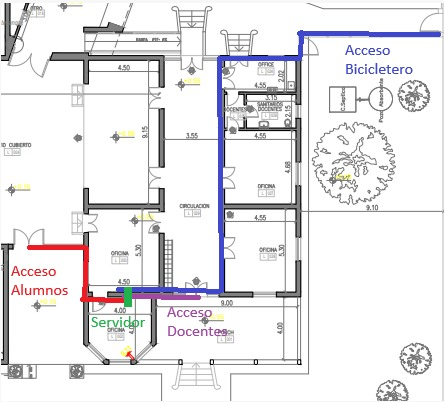
\includegraphics[width=1\textwidth]{img/Plano_Nuevo.jpeg}
	\caption{Plano de la institución resaltando los accesos y ubicación del servidor}
	\label{fig:plano}
\end{figure}


	\newpage
\section{Funcionamiento del sistema}
El sistema funciona en un horario determinado correspondiente al horario escolar. Por fuera de ese horario el sistema permanece inactivo y las puertas cerradas con llave.
Durante los horarios de ingreso, las puertas permanecen abiertas para evitar \enquote{cuellos de botella} por parte de los alumnos, pero una vez iniciado el periodo de clases, las puertas permanecen cerradas. Del lado de afuera se debe instalar un manijón que no permita que se accione el resbalón, ya que este lo acciona un destrabador eléctrico comandado por el sistema. Del lado interior se coloca un picaporte, que permita el egreso en todo momento por motivos de seguridad ante una posible evacuación.
En casos de fallas del suministro energético, cuando el destrabador no pueda accionarse, basta con accionar el resbalón desde dentro con el picaporte o desde fuera con la llave.

En caso de que un visitante externo, por ejemplo el tutor de un alumno, visite la escuela, al tocar el pulsador del timbre de alguna de las puertas se le toma una fotografía que llega al dispositivo movil de la persona a cargo, quien decide si comandar o no una apertura. El tibre sonoro debe seguir funcionando normalente.

El personal de la institución contará con credenciales de acceso en formato de tags NFC, con los que podrán acceder sin mediación humana. El sistema deberá llevar registro de cada acceso por cualquiera de los dos medios mencionados. 


\subsection{Arquitectura del sistema}
El sistema se compone de un nodo servidor implementado en una \textit{single board computer} (SBC) comunicado con tres nodos llamdados terminales, construidos en base a microcontroladores, ubicados físicamente en cada punto de acceso. El servidor gestiona las comunicaciones, los registros, los permisos de acceso y por supuesto, comanda a los terminales. Los terminales son los que comandan, bajo demanda del servidor, el desbloqueo de las puertas mediante sendos relés que accionan los destrabadores eléctricos. También controlan las cámaras que toman las fotografías del exterior y los sensores NFC para transmitir la información de estos al seridor. 

Existen dos canales de comunicación entre nodos:

\begin{itemize}
    \item Comunicación serial cableada mediante protocolo RS-485 para el flujo de comandos, configuraciones y eventos, ya que es un estandar robusto utilizado en la industria, de velocidades considerables y pensado para grandes distancias.
    \item Conexión a la red local, en el caso de los terminales via WiFi, mientras que el servidor puede conectarse via wifi o mediante cable de red si fuera posible, para transmitir las fotografías tomadas, dado que su transmición no es crítica en tiempo y que una fotografía se corresponde a un volumen de datos mayor que puede congestionar el canal principal.
\end{itemize}

 \begin{figure}[ht]
	\centering
	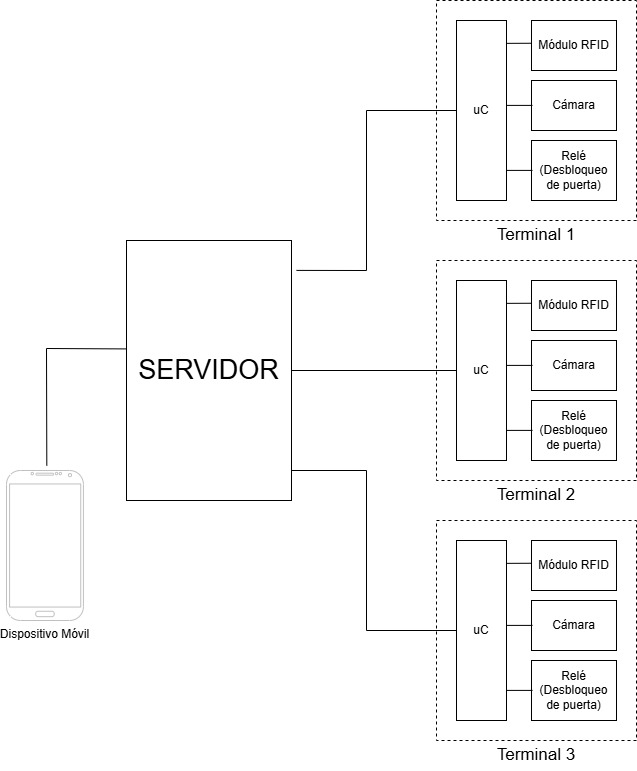
\includegraphics[width=0.7\textwidth]{img/DB1.jpeg}
	\caption{Diagrama de bloques del sistema}
	\label{fig:DB}
\end{figure}

\subsection{Actores del sistema}
El sistema reconoce tres tipos de actores humanos.

Los \textbf{accesos autorizados} son aquellos que cuenten con una credencial o \enquote{tag} nfc autorizado y puedan acceder al presentarlo frente al lector. El lector debe validar la identidad del tag mediante contraseña, recolectar la identificación y contador de accesos y enviarla al servidor, para que este contraste con la lista de tags permitidos y responda con la orden de apertura o de no apertura. El Funcionamiento de la lectura y validación se detalla en la sección (...).
El sistema debe tener capacidad para al menos 50 accesos autorizados, ya que representan al personal de la escuela (docente y no-docente) compuesto de alrededor de 30 personas. Se deja capacidad de reserva para cambios, incorporaciones y repuestos. 

Los \textbf{visiantes externos} son aquellas personas que no tienen autorización de ingresar fuera del horario de apertura. Estos, al pulsar el boton del timbre, son fotografiados por la cámara del terminal. La fotografía es enviada hacia el servidor, el cual lo envía hacia el dispositivo móvil donde un usuario final valida la identidad del visitante y concede o no el acceso. 

Los \textbf{usuarios finales} son aquellos con acceso a la interfaz de usuario de los dispositivos móviles. Para acceder a la interfaz estos deben loguearse con credenciales (usuario y contraseña). Según las credenciales pueden tener distintos roles. 
El más básico es el de usuario, cuya sesión permanece abierta en el dispositivo a menos que se cierre explícitamente o que se reabra en otro dispositivo. Este rol permite solo acciones básicas tales como comandar aperturas o solicitar fotografías. Este rol está dedicado al personal no docente, directivo o administrativo. El sistema admite hasta 6 usuarios con este rol.
Ciertos usuarios puden, mediante credenciales extra, abrir una sesión temporal de administrador, este rol permite configurar credenciales y añadir autorizaciones de accesos. Estas credenciales pertenecen solo a los directivos.
Finalmente, queda un rol de desarrollador al cual se accede con otras credenciales mediante un comando no disponible en el menú. Este rol no está pensado para el personal de la institución sino a quienes esten a cargo de la instalación y el mantenimiento del sistema, y permite realizar acciones simples sobre este sin la necesidad de acceder al servidor mediante SSH.

\subsection{Interfaces de usuario}

La interfaz principal para los usuarios finales funciona a travéz de un bot de la aplicación de mensajería instantanea \enquote{Telegram}, ya que la API es amigable con los desarrolladores y permite utilizar menúes y comandos de forma sencilla, además de que soluciona la conectividad con el exterior, sin tener que configurar manualmente puertos ni firewalls. Otra ventaja respecto a desarrollar una aplicación nativa es que no hay que hacer un desarrollo distinto para cada sistema operativo móvil.

El bot es en esencia un programa que se ejecuta permanentemente en el servidor y mediante llamadas a API recibe, procesa y envía mensajes al chat del bot.

Los registros históricos de accesos se dan en formatos legibles y se cargan diariamente a google drive mediante su API. Esto permite un fácil acceso a los datos y un ahorro de memoria del servidor al almacenar en la nube.

\subsection{Requerimientos del sistema}

Los requisitos temporales del sistema no son estrictos al punto de requerir una respuesta en tiempo real; sin embargo, el uso de este debe percibirse fluido para los actores.

Se establece entonces que el tiempo dé respuesta para los accesos autorizados debe estar en el orden de los dos segundos, contando desde que el tag se presenta ante el sensor hasta que se acciona el relé que destraba la puerta. 

En el caso del acceso de visitantes externos, el tiempo de respuesta se enmascara con la demora de la reacción humana, por lo que se establece una respuesta del orden de los cinco segundos del sistema para enviar la foto al usuario final, y del mismo orden para la apertura desde el comando manual, no pudendose controlar el tiempo de respuesta del usuario. 

Otro requerimiento es la robustez frente a fallas del suministro energético y la conexión a internet. Para eso se propone conectar el servidor a una unidad UPS para mantenerlo activo ante cortes de energía, aunque sin funcionamiento. El sistema se habilita solo en un horario determinado, en caso de un desfazaje del reloj del servidor, por ejemplo por un reinicio sin conexión a internet para ponerse en hora, se puede mediante un tag especial forzar el funcionamiento del sistema fuera de horario, al menos hasta que se retome la conectividad y el sistema vuelva a funcionar con normalidad.

El último requerimiento crítico es el de seguridad del sistema, el cual se abarca en la sección correspondiente (...).
	\section{Alcance del proyecto}
Se propone en el marco de este proyecto desarrollar un prototipo funcional que pueda ser adaptado a un entorno real como el de la problemática, incluyendo:

\begin{itemize}
	\item Construcción y programación de al menos un terminal incluyendo el microcontrolador, la cámara, el módulo RFID y las comunicaciónes contra el servidor.
	\item Programación del servidor incluyendo administración de comunicación multipunto, procesamiento de datos de entrada, historización de datos relevantes y programación de la comunicación con dispositivos externos.
	\item Comunicaciones de los dispositivos
	\item Escritura de tags para pruebas
\end{itemize}


Quedarán como mejoras a futuro el agregado de acceso remoto de mantenimiento fuera de red para el servidor, la migración de funcionalidades en medida de lo posible a lenguajes de mas bajo nivel para reducir el costo computacional y poder utilizar hardware mínimo y más económico, uso de algoritmos más sofisticados para reforzar la seguridad y la creación de perfiles alternativos de autorización  de acceso para extender el sistema a alumnos que entren fuera de horario en visión de escalar a una escuela inteligente.
	
	
\end{document}
